\chapter{Related Work}

\section{U-Net: Convolutional Networks For Biomedical
Image Segmentation} \label{unet}

    In this part, we introduce the architecture of the model that is the foundation of the work in this thesis, and hence in  more detailed. U-Net is a fully convolutional state-of-the-art\cite{rajak2021segmentation} semantic segmentation \gls{cnn} and was initially developed for biomedical image analysis by \citeauthor{unet_ronneberger2015}\cite{unet_ronneberger2015}. 
    
    \begin{figure}[H]
        \centering
        %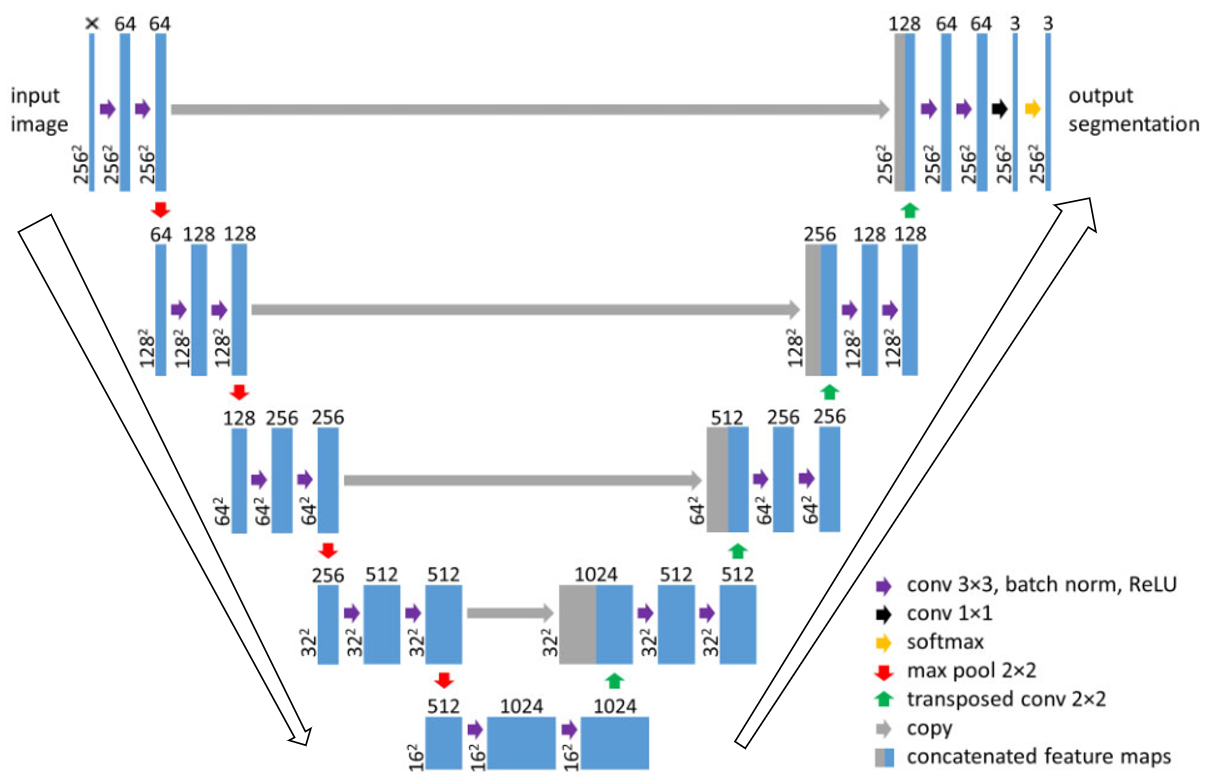
\includegraphics[scale=0.5]{figures/unet_arrows.png}
        \includesvg[inkscapelatex=false,width=1.0\textwidth,keepaspectratio]{figures/unet_original.svg}
        \caption[U-Net architecture]{U-Net architecture, the downwards facing arrow illustrates the contracting path and the one facing upwards is the expanding path. The color gets darker as the channels increase.}
      	\medskip 
        \label{unet_fig}
        \hspace*{15pt}\hbox{\scriptsize Credit: \citeauthor{unet_ronneberger2015}\cite{unet_ronneberger2015}}
    \end{figure}
    
    Unet utilized what \citeauthor{unet_ronneberger2015}\cite{unet_ronneberger2015} called a contracting path to identify what was in a picture, while an expanding path to localize where it was. These two branches were symmetrical, and together they formed a U-shape, giving the network its name. The contracting path can be looked at as five different stages of processing, from top to bottom, in figure \ref{unet_fig}. Each stage applied the same operations to its given input. For each stage, this consisted of two 3×3 valid convolutions with their individual ReLU activation functions. Initially, the feature channels would be increased to 64, and later doubled for each contracting stage. The convolutions were followed by a 2×2 max pooling operation with stride 2 to decrease the resolution of the output from the convolutional operations, and then send this feature map down to the next stage. At the bottom stage, the only change was the use of transpose convolutions instead of max pooling to now increase the resolution. At each subsequent stage going back up the expanding path, the number of feature channels were halved during the convolutional steps. The output of the previous stage would be concatenated with a crop from the output feature map of a stage from the contracting path with the same channel size, the cropping due to different resolutions. This step is crucial for the performance of the model, as it helps the network localize the abstract features in the expanding path to locations in the contracting. At the last stage, a 1×1 convolution was applied instead of increasing the resolution. The 1×1 convolution mapped the 64 feature channels to the 2 classes. The softmax was then calculated between these classes, giving each pixel a value between [0,1], summarized over all classes to 1. Hence, giving us a segmentation map of each class. In the field of biomedicine, data are scarce and so heavy use of data augmentation was applied, which made the U-Net able to train on very few samples.
    
    As of U-Net's development in \citeyear{unet_ronneberger2015}, it outperformed other networks in multiple biomedical challenges\cite{unet_ronneberger2015}. It's performance inspired new versions with enhanced performance that use the U-Net architecture as its backbone, as can be seen in NAS-Unet\cite{weng2019unet} from \citeyear{weng2019unet}, and Unet++\cite{zhou2018unet} from \citeyear{zhou2018unet}. U-Net has also been applied with success to other fields such as road extraction in satellite images by \citeauthor{zhang2018road}\cite{zhang2018road} in \citeyear{zhang2018road} and on acoustic classification by \citeauthor{brautaset2020acoustic}\cite{brautaset2020acoustic} in \citeyear{brautaset2020acoustic}, which is the next article to be described in this thesis.
    
    
\section{Acoustic Classification In Multifrequency Echosounder Data Using Deep Convolutional Neural Networks} \label{unet_paper_acoustic}
    
        \begin{figure}[H]
        \centering
        %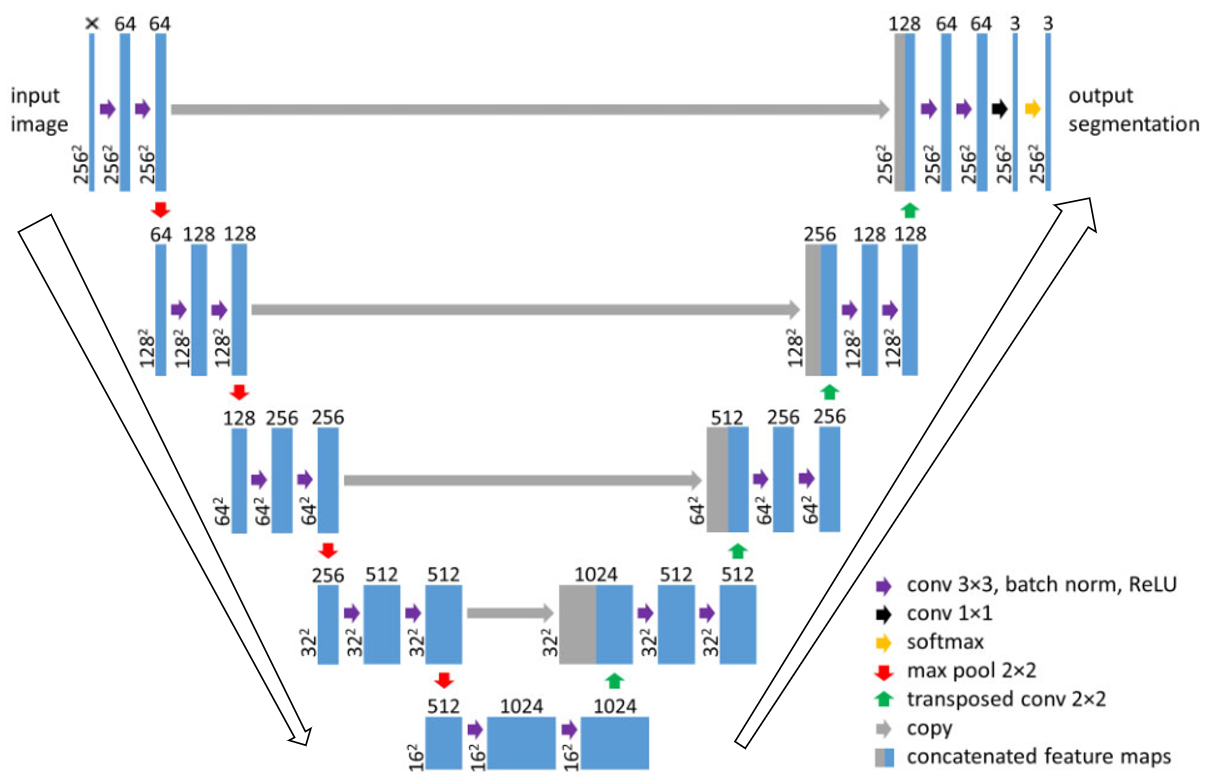
\includegraphics[scale=0.5]{figures/unet_arrows.png}
        \includesvg[inkscapelatex=false,width=1.0\textwidth,keepaspectratio]{figures/unet_brautset.svg}
        \caption[U-Net architecture]{U-Net architecture, the downwards facing arrow illustrates the contracting path and the one facing upwards is the expanding path. The color gets darker as the channels increase.}
      	\medskip 
        \label{unet__brautset_fig}
        \hspace*{15pt}\hbox{\scriptsize Credit: \citeauthor{brautaset2020acoustic}\cite{brautaset2020acoustic}}
    \end{figure}
    
    
    \citeauthor{brautaset2020acoustic}\cite{brautaset2020acoustic} had as objective to propose a deep learning method to classify and segment acoustic data gathered during acoustic trawl surveys, without using predefined features. This work is the backbone of this thesis and the data is the same or very similar, hence a more detailed description is provided. The acoustic data from the surveys are used as support when fisheries estimate the allowed catches of different fish populations, and in this case \textit{sand eel}. To estimate the quantity of fish, there is a linear relationship between the \gls{sv} value and quantity as long as the exact species can be assigned to the value. Today, the process of designating \gls{sv} to the proper species is heavily influenced by human operators using a variety of tools, and trawl samples (biological samples). These tools use predefined features, and are subject to not fit all situations equally well. 
    
    The deep learning architecture proposed was based on an altered version of \citeauthor{unet_ronneberger2015}\cite{unet_ronneberger2015} U-Net\cite{brautaset2020acoustic}. It is visualized in figure \ref{unet__brautset_fig}, and the difference is the use of \textit{same convolutions} and \textit{batch normalization}. Furthermore, as the resolution of the layers in the contracting and expanding path had the same size, when concatenating, cropping was no longer needed. 
    
    The data used originated from yearly trawl missions spanning 2007-2018\cite{brautaset2020acoustic}, where 2011-2016 was set as training and validation data, and 2007-2010 combined with 2017-2018 as test data. The frequency channels extracted from each year was the 18kHz, 38kHz, 70kHz and 200kHz. Operator annotations initially contained the classes \textbf{sandeel}, \textbf{other}, \textit{0-group sandeel} and \textit{possible sandeel}, and were annotated by the same operator. \textit{0-group sandeel} and \textit{possible sandeel} was added to a new class \textbf{ignore}, as both of them were edge cases, originated from an extraordinary event seen during a trawl or operator uncertainty. The annotations were converted to a pixel map of the same size as the \gls{sv} data, and all pixels not allocated to a class was set as the \textbf{background class}. Annotations were originally designed to summarize the \gls{sv} values over an area, to estimate quantity. Hence, they were usually square and larger than the actual school of fish, and not suitable as labels for a \gls{cnn} due to some pixel around the edges really belonging to the \textit{background class}. As a result, the annotations were approximately reshaped to be more similar to real schools of fish. The outline of further methods applied is described in the methodology section (section \ref{methods}) as it is based on this article.
    
    Performance was measured using two different methods\cite{brautaset2020acoustic}. The first method extracted predictions in \textbf{small regions} around existing annotations, and was applied due to  the observations of many schools lacking annotations. This would likely result in the decrease of many false positives being produced by the model, and would now reflect its actual performance. The second method was to measure the performance over \textbf{entire echograms}. A current benchmark method was also applied to compare performance. The metric used was F1-score, where \textit{sandeel} was the \textbf{positive}   while \textit{other} and \textit{background} was the \textbf{negative}. \textbf{Small regions} resulted in an overall F1-score of 0.87 on all the test data after a threshold of 0.8 was applied to the probabilities, while the benchmark achieved a F1 score of 0.77. When applying the model to \textbf{entire echograms}, the performance decreased and ranged from 0.11-0.68 on individual test years. This was also mirrored by the benchmark method, which achieved 0.03-0.50. The decrease in performance was attributed to missing annotations, and many factors causing high \gls{sv} values but being allocated to the \textit{background} class and due to the training scheme rarely, if ever, seen by the model. The quality of the data from different years varied due to different weather conditions, fish populations and stages of development in software used during annotations. The conclusion was that the model was able to be reliably trained to classify acoustic multifrequency measurements\cite{brautaset2020acoustic}.
    
    
%    - goal, (i) develop a deep learning
%        strategy that is suitable
%        for segmenting and classifying echosounder data collected during acoustic trawl surveys %without prior feature extraction; (ii) demonstrate that the strategy devel-
%        oped in (i) works on a real test case, and (iii) provide perspec- tives, e.g. pros and %cons, on the use of deep learning algorithms in the classification of acoustic %observations into acoustic catego-ries (e.g. species groups).



% - modified architecture, same convs, batch norm
% - trawl missions from 2007 - 2018, many classes, combined into three
% - four frequencies used -> output segmantation map of sandeel, other and background
% - preprocessing of the data, as we use the same approach this is described in the %AC-tool.
%    - regrid to 200kHz
% - modified the annotations to be more similar to actual schools of sandeel
% - balanced sampling 256x256x4 crops with regard to the information contained in the crop % equal probability from the dataset
% - a word about the classes.
% - a thing about the annotations, not deemed fully compatible with semantic segmentation, one %ator
%- Performance
%    - Training scheme outlined in the methodology, 
%    - stained by domain knowledge, and there could be more imacting performance
%        - when calculating F1 score, compare only examined regions withing 20 pixels of an actual annoation (false positive)
%        - 0.87 F1 at discriminate between sandeel (positive) and background and other as negative across the test data. Benchmark method got 0.77.
%        
%    - When evaluating entire echograms, was deem satisfactory for 2018 and 2017 at 0.78 and 0.68, benchmark (0.62 and 0.32)
%    - Both on complete echograms,unet (0.11 - 0.68) and 0.03-0.5)
%
%Echograms contain (problems): 
%- missing annotations, will confuse a pixel based classifier as there were clear signs of sandeel
%- false positives near the surface as, and was speculated to be dense layers of plankton, resulting in high sv values hence being classified as sandeel, and was missed was not data the model had been exposed to earlier. (this causes my model to likely classify this as sandeel). The exact plankton "Phaeocystis" produces gases which have high intensity at 18 and 38kHz, and could be a reason why the. The backround class contains everything not related to the other and sandeel class so will maybe contain other noise inducing factors, as seen when trying to predict entire echograms  
%
%- large uncertainy across years, weather conditions and school populations,  which affects %the quality quality of labeling. Historical data was affected by tools being under %development.
    
    
    
    
    
    
    %OBS! Må ha forklart U-net, accoustic klassifikasjon, F1 OBS, feature construction, statistical and machine learning methods!
    
    %To help assess the size of legal fishing quotas, acoustic trawls surveys are initiated to gather data. Before the data is of use, an operator manually needs to interpret the data in a time-consuming process to assign the acoustic back scattering to the correct category, but in turn often introduces bias. Several methods have been implemented to reduce this bias and with a goal to automate the process, but they all have a common weakness where they need a predefined feature space.  In 2020 a group of researchers implemented a U-net deep learning model to the problem and as this is an \gls{cnn} it does not need to have pre-designed features but learn them from the data. Sandeel  ~\cite{brautaset2020acoustic}. 
    
    %In this thesis, this will be a semantic segmentation of the classes \textit{background}, \textit{other } and most importantly \textit{sandeel}.
    
    
    
    %The \gls{crimac} used this model in their project (described in \ref{unet_paper_acoustic}) and had to do some small modifications to the network to fit their task. This modified U-Net is the one presented in this section, as this is the one used in the experiments. The core functionality of the network stays true to the original Unet, and the alterations done to the original will be explained later in this section.
    
    
    
    
    %Minor changes were made to adapt\citeauthor{unet_ronneberger2015}s original U-Net to the acoustic data used in \ref{unet_paper_acoustic}, as the input now had the form 4 x 256 x 256. The four channels being the frequencies used. The convolutions were set to \textit{same} instead of \textit{valid}, as were the original setting. This was done to make the size of the input and output match. Further, batch normalization was added to each convolution. 
    
 
 
 

    @article{Marques2021InstanceSI,
  title={Instance Segmentation-based Identification of Pelagic Species in Acoustic Backscatter Data},
  author={Tunai Porto Marques and Melissa Cote and Alireza Rezvanifar and Alexandra Branzan Albu and Kaan Ersahin and Todd Mudge and St{\'e}phane Gauthier},
  journal={2021 IEEE/CVF Conference on Computer Vision and Pattern Recognition Workshops (CVPRW)},
  year={2021},
  pages={4373-4382}
}
- instance segmentation
- automate the process, automatic bilogical analysis

